%\vspace{1.5pc}
\vspace{1.5pc}
\section[Aplikasi pada \textit{Bay of Bengal} (BoB)]{Aplikasi pada \textit{Bay of Bengal}  (BoB)}
\begin{spacing}{1.5}
\vspace{-1pc}
\subsection[Sirkulasi Arus dan Angin]{Sirkulasi Arus dan Angin}
	
	Gambar \ref{fig:arus} menunjukkan plot arus rata-rata (u dan v) di BoB di atas permukaan laut untuk bulan Januari dan Juli 2021. Warna pada gambar mewakili elevasi permukaan air laut (dalam meter) dan vektor arah sebagai sirkulasi permukaan laut (dalam m/s). Pada bulan Januari (Gambar \ref{fig:arus}(a)), arus permukaan lebih kuat di sepanjang batas terbuka (\textit{open boundaries}) dan di beberapa area di mana pusaran (\textit{eddies}) terjadi. Tiga pusaran tampak sangat menonjol pada koordinat ($82^\circ$E, $12^\circ$N), ($87^\circ$E, $19^\circ$N), dan ($95^\circ$E, $8^\circ$N) yang ditandai dengan arah arus yang berbeda dan nilai elevasi permukaan yang kontras. \textit{Eddy} pada koordinat ($82^\circ$E, $12^\circ$N) memiliki arah berlawanan jarum jam dan elevasi permukaan yang rendah, $0.3 - 0.4$ m. Sebaliknya, \textit{eddy} pada koordinat ($87^\circ$E, $19^\circ$N) memiliki arah searah jarum jam dan elevasi permukaan yang tinggi, $0.6 - 0.7$ m. Arah arus searah jarum jam juga terjadi dengan \textit{eddy} pada koordinat ($95^\circ$E, $8^\circ$N) dan dengan elevasi permukaan $0.55 - 0.6$ m
	
	Pada bulan Juli (Gambar \ref{fig:arus}(b)), arus permukaan yang diamati juga menunjukkan arus yang kuat di sepanjang batas terbuka dan di beberapa daerah di mana pusaran terjadi. Terlihat bahwa 2 pusaran yang sangat menonjol pada bulan Juli berada pada koordinat ($83^\circ$E, $14^\circ$N) dan ($83^\circ$E, $16^\circ$N) yang juga ditandai dengan arah arus yang berbeda dan nilai elevasi permukaan yang kontras. Eddy pada koordinat ($83^\circ$E, $14^\circ$N) memiliki arah searah jarum jam dan elevasi permukaan yang tinggi, $0.6 - 0.7$ m. Di sisi lain, eddy pada koordinat ($83^\circ$E, $16^\circ$N) memiliki arah berlawanan jarum jam dan elevasi permukaan yang rendah, $0.3$ m.
	
	\begin{figure}[H]
		\centering
		\includegraphics[width=14.5cm]{contents/final_figure/Figure_2}
		\caption{Elevasi permukaan laut (warna dalam meter) dan sirkulasi permukaan laut (panah dalam m/s) pada (a) Januari dan (b) Juli 2021, data dari HYCOM.}
		\label{fig:arus}
	\end{figure}

	Arus pada Gambar \ref{fig:arus} dipengaruhi oleh berbagai faktor, salah satunya adalah angin. Angin ditunjukkan pada Gambar \ref{fig:angin} untuk pembahasan lebih lengkap. Stres atau tekanan angin diwakili oleh panah (dalam Pa), dan gradasi warna mewakili kecepatan angin (dalam m/s). Pada bulan Januari (Gambar \ref{fig:angin}(a)) angin bertiup dari arah timur laut ke arah barat daya, sedangkan pada bulan Juli (Gambar \ref{fig:angin}(b)) angin bertiup dari arah barat daya menuju timur laut.
	
	\begin{figure}[H]
		\centering
		\includegraphics[width=14cm]{contents/final_figure/Figure_3}
		\caption{Kecepatan angin (warna dalam m/s) dan tekanan angin (panah dalam Pa) pada (a) Januari dan (b) Juli 2021, data dari NCEP/NCAR.}
		\label{fig:angin}
	\end{figure}
	
	Secara umum kondisi angin pada bulan Januari mengakibatkan kecenderungan arus bergerak dari timur ke barat pada batas buka selatan. Mayoritas arus untuk bulan Januari lebih kuat di batas terbuka dan di pantai. Arus yang juga kencang terpantau karena letak pusaran air dekat dengan pantai.
	
	Sebaliknya, kondisi angin pada bulan Juli mengakibatkan arus cenderung bergerak dari barat ke timur pada batas buka selatan. Sebagian besar arus untuk bulan Juli lebih kuat di dekat pantai barat BoB karena pusaran arus yang kuat. Pada kedua bulan tersebut, kecepatan arus pada lokasi batas terbuka dan pusaran dapat mencapai 1 m/s.
	
\subsection[Profil Transek Vertikal]{Profil Transek Vertikal}
	
	Penampang temperature (\textit{cross-sectional temperature}) digunakan dalam penelitian ini untuk memberikan ide dan deskripsi mengenai lokasi gradien temperature tertinggi untuk memberikan hasil yang lebih komprehensif. Penampang temperature disajikan pada Gambar \ref{fig:mld} untuk melihat kedalaman lapisan campuran (MLD) di bagian selatan BoB (lintang $9^\circ$N) dan utara BoB (lintang $19^\circ$N) selama 12 bulan. Estimasi kedalaman MLD dari Gambar \ref{fig:mld} disajikan pada Tabel \ref{table:MLD_thickness} sebagai bahan pelengkap pembahasan.
	
	Kriteria yang digunakan untuk menggambarkan MLD dalam peta pada Gambar \ref{fig:mld} adalah nilai ambang suhu (\textit{threshold}) $0.1^\circ$C. Citra penampang diplot terlebih dahulu tanpa kontur dengan menggunakan kriteria ini untuk menghasilkan citra dengan warna berbeda yaitu merah, putih, dan biru. Gambar kontur kemudian ditambahkan untuk melihat nilai temperature. Indikator nilai ketebalan MLD berdasarkan temperature $25^\circ$C dengan warna merah muda pada gambar. Gambar \ref{fig:mld} menunjukkan penampang temperature lautan (dalam $^\circ$C) pada garis lintang $9^\circ$N dan garis lintang $19^\circ$N selama 12 bulan pada tahun 2021. Penampang dijelaskan menggunakan hubungan antara bujur atau longitude (sumbu x, dalam derajat) dan kedalaman (sumbu y, dalam meter). Nilai suhu bervariasi berdasarkan bujur dan kedalaman. Ini digambarkan oleh kontur dan bilah warna (\textit{colorbar}). Bilah warna ditetapkan dari rentang nilai $0 - 30^\circ$C, dan kedalamannya dibatasi dari $0-150$ meter agar gambar dapat dengan mudah dibaca.
	
	\begin{figure}[H]
		\centering
		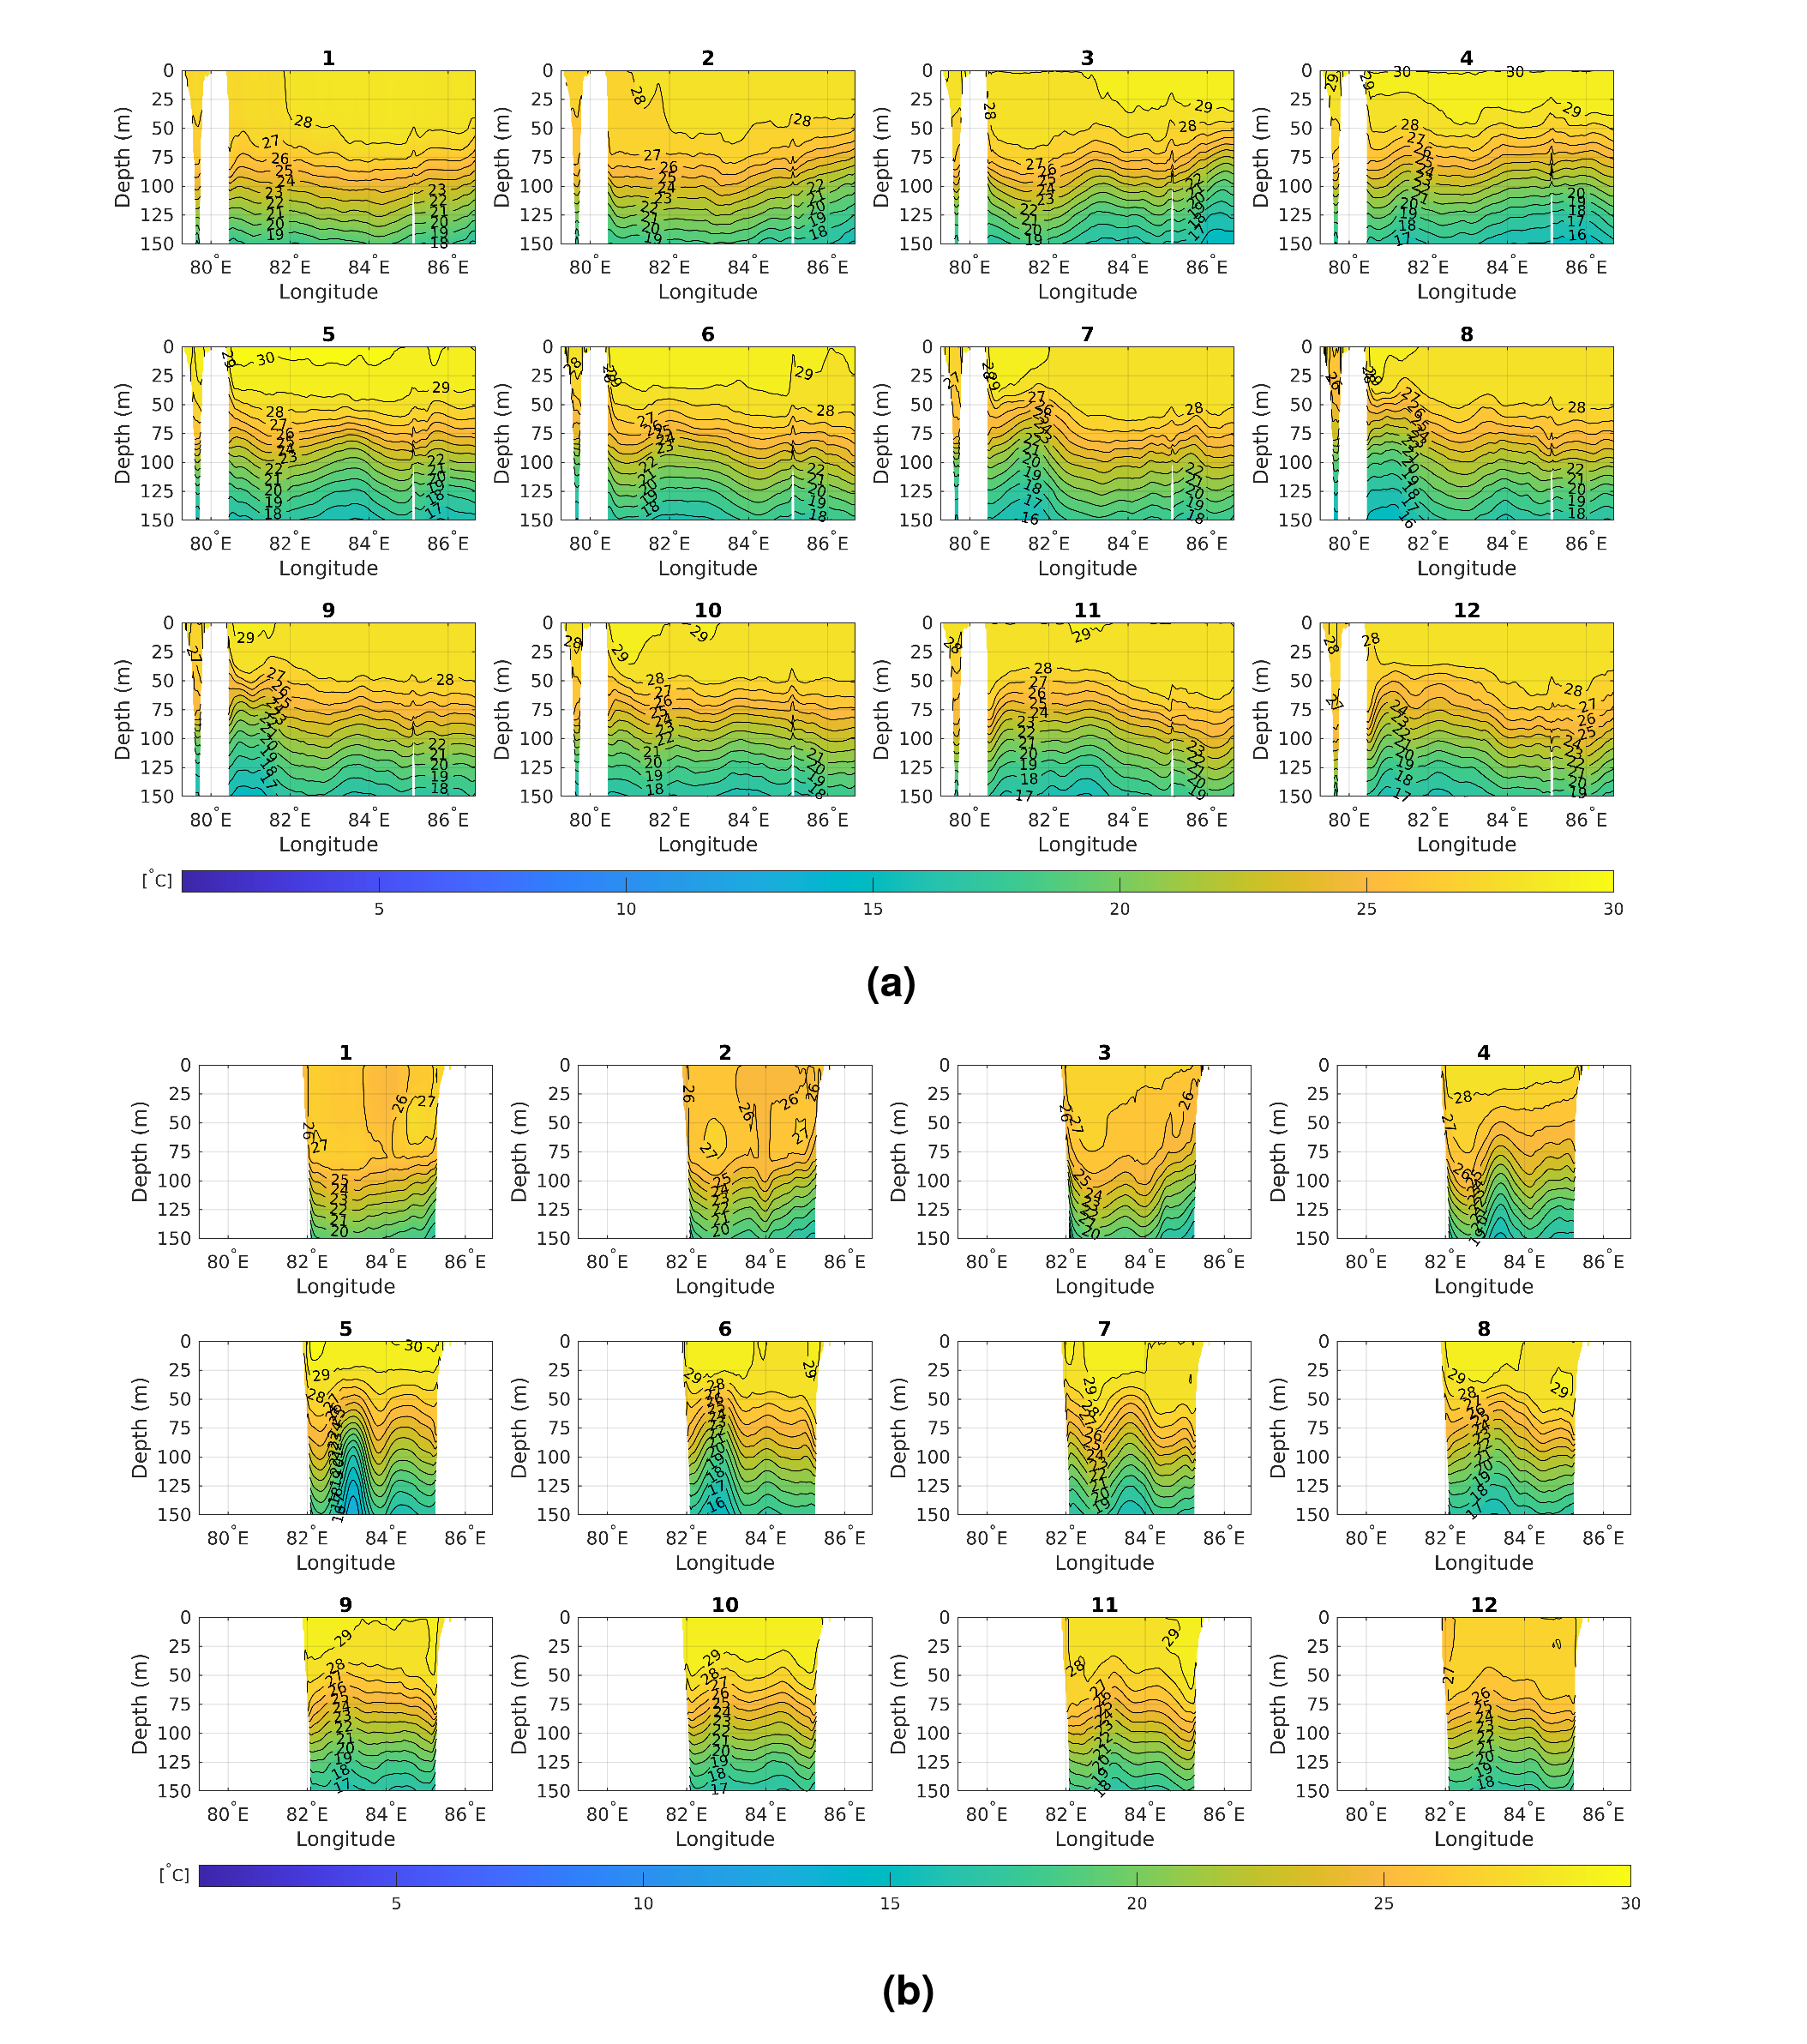
\includegraphics[width=16cm]{contents/final_figure/Figure_4}
		\caption{Penampang temperature lautan pada (a) garis lintang $9^\circ$N dan (b) garis lintang $19^\circ$N pada tahun 2021 (12 bulan), diperoleh dari HYCOM (https://www.hycom.org/).}
		\label{fig:mld}
	\end{figure}
	
	Pada bagian selatan BoB, Gambar \ref{fig:mld}(a) menunjukkan adanya 3 warna yang sangat kontras, yaitu merah, merah muda, dan putih. Hal ini menunjukkan bahwa nilai suhu pada kedalaman 0 sampai 150 meter bervariasi antara $15^\circ$C sampai $30^\circ$C. Pada kedalaman $0-50$ m, nilai suhu berkisar antara $28^\circ$C hingga $30^\circ$C dan mendominasi di semua bulan. Ini ditandai dengan warna merah, dan kontur pada gambar. Pada kedalaman $50-100$ m, nilai suhu berkisar antara $23^\circ$C hingga $28^\circ$C yang ditandai dengan warna merah muda. Pada kedalaman $100-150$ m, nilai suhu berkisar antara $16^\circ$C hingga $23^\circ$C yang ditandai dengan warna putih.
	
	Perbedaan 3 warna yang kontras (merah, merah muda, dan putih) juga terjadi di bagian utara BoB, Gambar \ref{fig:mld}(b). Pada kedalaman $0-50$ m, nilai suhu berkisar antara $27^\circ$C hingga $30^\circ$C yang ditandai dengan warna merah dan kontur pada gambar. Pada kedalaman $50-100$m, nilai suhu berkisar antara $24^\circ$C hingga $27^\circ$C, kecuali beberapa bulan terakhir (September hingga Desember) yang dapat mencapai sekitar $22^\circ$C hingga $27^\circ$C. Ini ditandai dengan merah muda pada gambar. Terakhir, pada kedalaman $100 - 150$ m, nilai suhu berkisar antara $16^\circ$C hingga $24^\circ$C dari Januari hingga Agustus dan $17^\circ$C hingga $22^\circ$C dari September hingga Desember, yang ditandai dengan warna putih. Nilai MLD dalam Tabel \ref{table:MLD_thickness} diperkirakan dari Gambar 4 berdasarkan temperature $25^\circ$C dengan warna merah muda sebagai indikasi MLD ketebalan.

	\begin{table}[H]
		\centering
		\caption{Estimasi ketebalan MLD (dalam meter) selama 12 bulan pada tahun 2021}
		\label{table:MLD_thickness}
		\resizebox{\columnwidth}{!}{%
			\begin{tabular}{|c|cccccccccccc|}
				\hline
				\multicolumn{1}{|c|}{\multirow{2}{*}{Domain}} & \multicolumn{12}{c|}{Months}                                                                                                                                                                                                                                                                                                                                      \\ \cline{2-13} 
				\multicolumn{1}{|c|}{}                        & \multicolumn{1}{l|}{1}        & \multicolumn{1}{l|}{2}        & \multicolumn{1}{l|}{3}        & \multicolumn{1}{l|}{4}        & \multicolumn{1}{l|}{5}       & \multicolumn{1}{l|}{6}       & \multicolumn{1}{l|}{7}       & \multicolumn{1}{l|}{8}       & \multicolumn{1}{l|}{9}       & \multicolumn{1}{l|}{10}      & \multicolumn{1}{l|}{11}       & 12      \\ \hline
				Latitude $9^\circ$N                                   & \multicolumn{1}{l|}{75-90m}  & \multicolumn{1}{l|}{70-100m} & \multicolumn{1}{l|}{60-95m}  & \multicolumn{1}{l|}{70-95m}  & \multicolumn{1}{l|}{70-85m} & \multicolumn{1}{l|}{70-85m} & \multicolumn{1}{l|}{65-90m} & \multicolumn{1}{l|}{65-85m} & \multicolumn{1}{l|}{65-80m} & \multicolumn{1}{l|}{65-80m} & \multicolumn{1}{l|}{70-100m} & 60-95m \\ \hline
				Latitude $19^\circ$N                                  & \multicolumn{1}{l|}{80-100m} & \multicolumn{1}{l|}{60-100m} & \multicolumn{1}{l|}{50-105m} & \multicolumn{1}{l|}{65-105m} & \multicolumn{1}{l|}{50-85m} & \multicolumn{1}{l|}{50-95m} & \multicolumn{1}{l|}{65-85m} & \multicolumn{1}{l|}{60-85m} & \multicolumn{1}{l|}{70-85m} & \multicolumn{1}{l|}{75-85m} & \multicolumn{1}{l|}{75-100m} & 75-85m \\ \hline
			\end{tabular}%
		}
		\raggedright
		\tiny
		
	\end{table}
		
		Berdasarkan indikator ketebalan MLD yang telah ditentukan sebelumnya, estimasi nilai ketebalan MLD dapat diperoleh pada Tabel \ref{table:MLD_thickness}. Nilai ketebalan MLD dibuat menggunakan interval ini untuk mengakomodasi nilai ketebalan yang bervariasi berdasarkan garis bujur yang berbeda. Tabel \ref{table:MLD_thickness} menunjukkan bahwa nilai MLD pada garis lintang $9^\circ$N dapat memiliki nilai ketebalan yang bervariasi mulai dari 60 m hingga 100 m. Terlihat bahwa variasi ketebalan MLD sepanjang garis bujur cukup besar pada bulan Maret dan Desember, yaitu dapat mencapai 35 m. Juga, bulan ini, MLD paling dangkal terjadi di 60 m. MLD terdalam ditunjukkan pada bulan Februari dan November, yaitu 100 m.
		
		Di sisi lain, garis lintang $19^\circ$N pada Tabel \ref{table:MLD_thickness} menunjukkan bahwa ketebalan MLD bervariasi dari 50 m hingga 105 m. Variasi ketebalan MLD sepanjang garis bujur dapat mencapai 55 m yang terjadi pada bulan Maret. Terlihat pula nilai MLD terdangkal terjadi pada bulan Maret, Mei, dan Juni yaitu 50 m, sedangkan MLD terdalam ditunjukkan pada bulan Maret dan April yaitu 105 m. Misalkan nilai variasi MLD di kedua garis lintang dirata-ratakan. Pada kasus tersebut, lintang $19^\circ$N menunjukkan variasi ketebalan MLD yang paling besar yaitu 28.3 m, dibandingkan dengan variasi ketebalan MLD pada lintang $9^\circ$N yang hanya 23.3 m. 
		
		\begin{table}[H]
			\centering
			\caption{Ketebalan MLD rata-rata (dalam meter) berdasarkan Monsun}
			\label{table:MLD_monsoon}
			\begin{tabular}{|c|cc|cc|}
				\hline
				\multirow{2}{*}{Domain} & \multicolumn{2}{c|}{Winter (Nov-Feb)} & \multicolumn{2}{c|}{Summer (Jun-Sep)} \\ \cline{2-5} 
				& \multicolumn{1}{c|}{MinX}   & MaxX  & \multicolumn{1}{c|}{MinX}   & MaxX  \\ \hline
				Latitude $9^\circ$N             & \multicolumn{1}{c|}{68.75}   & 96.25  & \multicolumn{1}{c|}{66.25}   & 85     \\ \hline
				Latitude $19^\circ$N            & \multicolumn{1}{c|}{72.5}    & 96.25  & \multicolumn{1}{c|}{61.25}   & 87.5   \\ \hline
			\end{tabular}
		\end{table}

		Ketebalan MLD rata-rata dalam Tabel \ref{table:MLD_monsoon} dihitung dari Tabel \ref{table:MLD_thickness} dengan rata-rata ketebalan minimum dan maksimum lapisan MLD berdasarkan musim. Tabel \ref{table:MLD_monsoon} menyajikan nilai rata-rata batas bawah (MinX) dan batas atas (MaxX), pada garis lintang $9^\circ$N dan $19^\circ$N pada bulan-bulan monsun musim dingin (November-Februari) dan bulan-bulan monsun musim panas (Juni-September).
		
		Rumus yang digunakan untuk mencari nilai Min dan Max adalah sebagai berikut
		\begin{equation*}
			\text{MinX}=\frac{\sum_{i=\{\{11,12,1,2\},\{6,7,8,9\}\}}\text{MinX}_i}{4}, \quad
			\text{MaxX}=\frac{\sum_{i=\{\{11,12,1,2\},\{6,7,8,9\}\}}\text{MaxX}_i}{4}
		\end{equation*}
	
		Dengan $i$ adalah jumlah bulan-bulan monsun musim dingin (Nov-Feb) atau musim panas (Jun-Sep). Tabel \ref{table:MLD_monsoon} menunjukkan bahwa ketebalan lapisan MLD lebih tebal pada musim dingin dibandingkan musim panas, baik untuk kedalaman minimum maupun maksimum. Ini berlaku untuk lintang $9^\circ$N dan lintang $19^\circ$N.
	
\subsection[Hubungan antara Parameter Meteorologi]{Hubungan antara Parameter Meteorologi}
	
		Terdapat beberapa gaya atmosfer dievaluasi untuk menerangkan perilaku MLD yang dianalisis dari model HYCOM, lima di antaranya adalah temperature udara 2m (AirT), kelembaban spesifik 2m (SHum), laju presipitasi konvektif (CPrecR), tekanan permukaan laut (SLP), dan tekanan angin (TauX dan TauY). Gambar \ref{fig:ncep_1} dan \ref{fig:ncep_2} menunjukkan hasil visualisasi dari kelima gaya tersebut selama 20 tahun dari tahun 2002 hingga 2021 di bagian selatan BoB (lintang $9^\circ$N) dan bagian utara BoB (lintang $19^\circ$N). Gambar ini dihasilkan dari data \textit{reanalysis} NCEP, yang dapat diunduh di https://psl.noaa.gov/.
		
		Nilai ekstrim tahunan dari lima gaya atmosfer untuk dua domain penelitian (lintang $9^\circ$N dan lintang $19^\circ$N) ditunjukkan pada Table \ref{table:NCEP_9} dan \ref{table:NCEP_19} (Lampiran 1). Tabel ini berguna untuk menentukan puncak dan lembah dari setiap parameter meteorologi. Gambar \ref{fig:ncep_1} dan \ref{fig:ncep_2} dimaksudkan untuk melihat perulangan (periodesitas) dari 5 parameter yang diteliti. Sedangkan Tabel \ref{table:NCEP_9} dan \ref{table:NCEP_19} diturunkan dari Gambar \ref{fig:ncep_1} dan \ref{fig:ncep_2}. Tabel ini berfungsi untuk melihat data secara kuantitatif. Nilai ekstrim ini penting untuk melihat pada bulan apa saja nilai ekstrim tersebut terjadi, dan ini dijadikan acuan untuk melihat parameter meteorologi yang mempengaruhi terjadinya nilai ekstrim tersebut.
		
		Secara keseluruhan, tren dari ketiga variabel AirT, SHum, dan tekanan angin (TauX dan TauY) memiliki nilai minimum pada musim dingin atau Desember-Februari dan nilai maksimum pada akhir musim semi dan musim panas pada bulan Mei-Agustus. Di sisi lain, tren dua variabel yang tersisa yaitu CPrecR dan SLP memiliki nilai minimum pada akhir musim semi dan musim panas, atau Mei-Juli, dan nilai maksimum pada musim dingin, dari Desember-Februari.
		
		Tercatat bahwa, pada lintang $9^\circ$N, nilai rata-rata minimum dari lima variabel adalah $25.47, 0.015, -0.0003, 100.2, -0.15$, dan $-0.11$ untuk setiap unit. Sedangkan nilai rata-rata maksimum dari kelima variabel berturut-turut adalah $30.53, 0.022, 0, 101.61,$ $0.225$, dan $0.18$ untuk setiap unit. Apabila nilai ekstrim pada lintang $9^\circ$N dibandingkan dengan nilai ekstrim pada lintang $19^\circ$N, selisih selang minimum dan maksimum pada lintang $19^\circ$N lebih besar dibandingkan pada lintang $9^\circ$N. Akibatnya adalah antara dua domain yang diteliti, nilai ekstrim yang lebih besar terjadi pada garis lintang $19^\circ$N. Selanjutnya, pada garis lintang $19^\circ$N nilai rata-rata minimum untuk kelima variabel adalah $20.99, 0.009, -0.0004, 99.57,$ $-0.11, -0.11$ untuk setiap unit, sedangkan rata-rata nilai maksimum untuk kelima variabel adalah $31.2, 0.023, 0.102, 0.196 , 0.231$ untuk setiap unit.
		
		\begin{figure}[H]
			\centering
			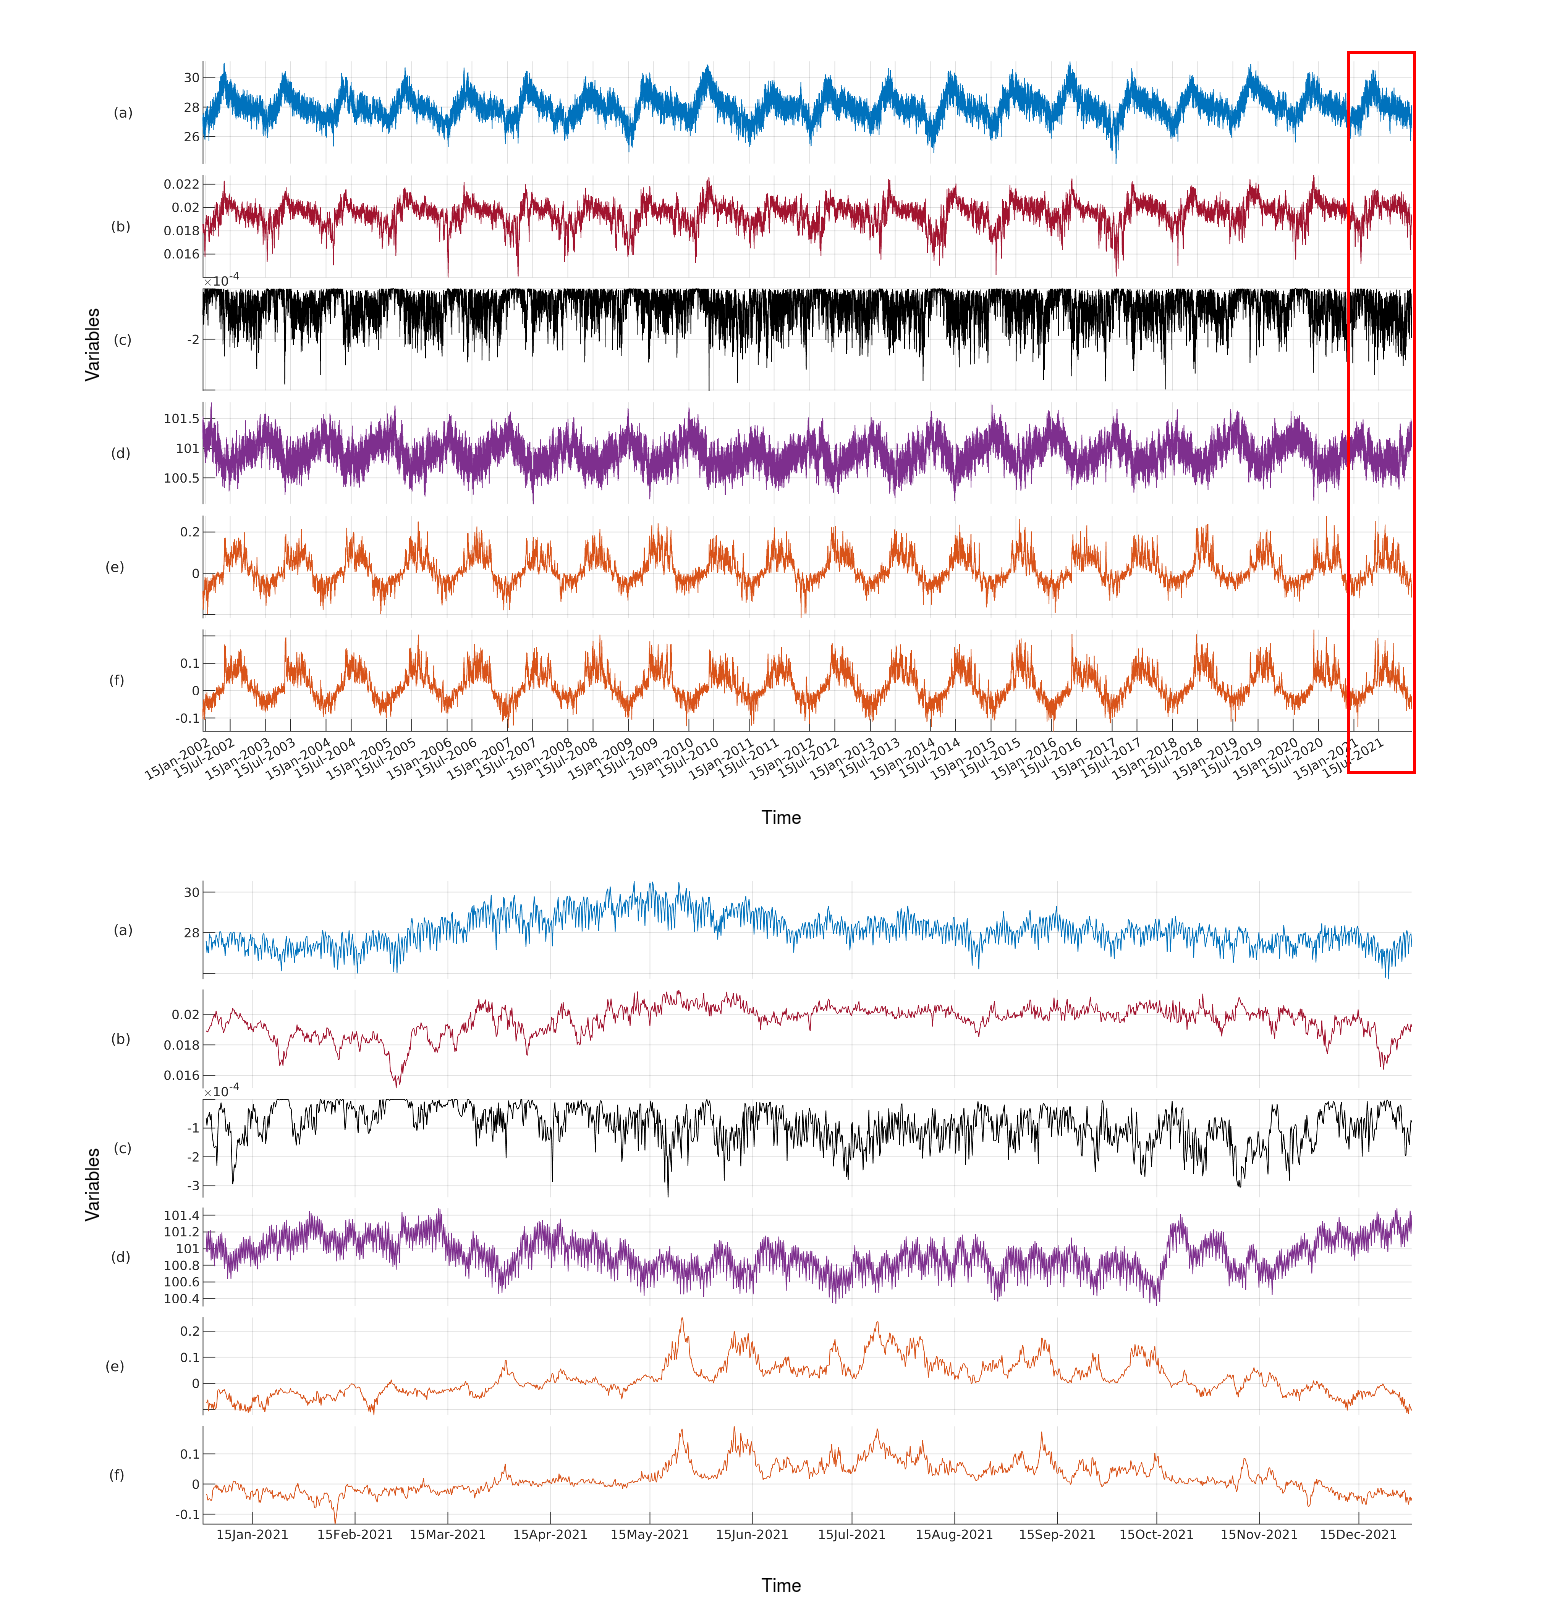
\includegraphics[width=16cm]{contents/final_figure/Figure_5a}
			\caption{Gaya atmosfer pada garis lintang $9^\circ$N dari tahun 2002 hingga 2021, data dari NCEP/NCAR.}
			\label{fig:ncep_1}
		\end{figure}
	
		\begin{figure}[H]
			\centering
			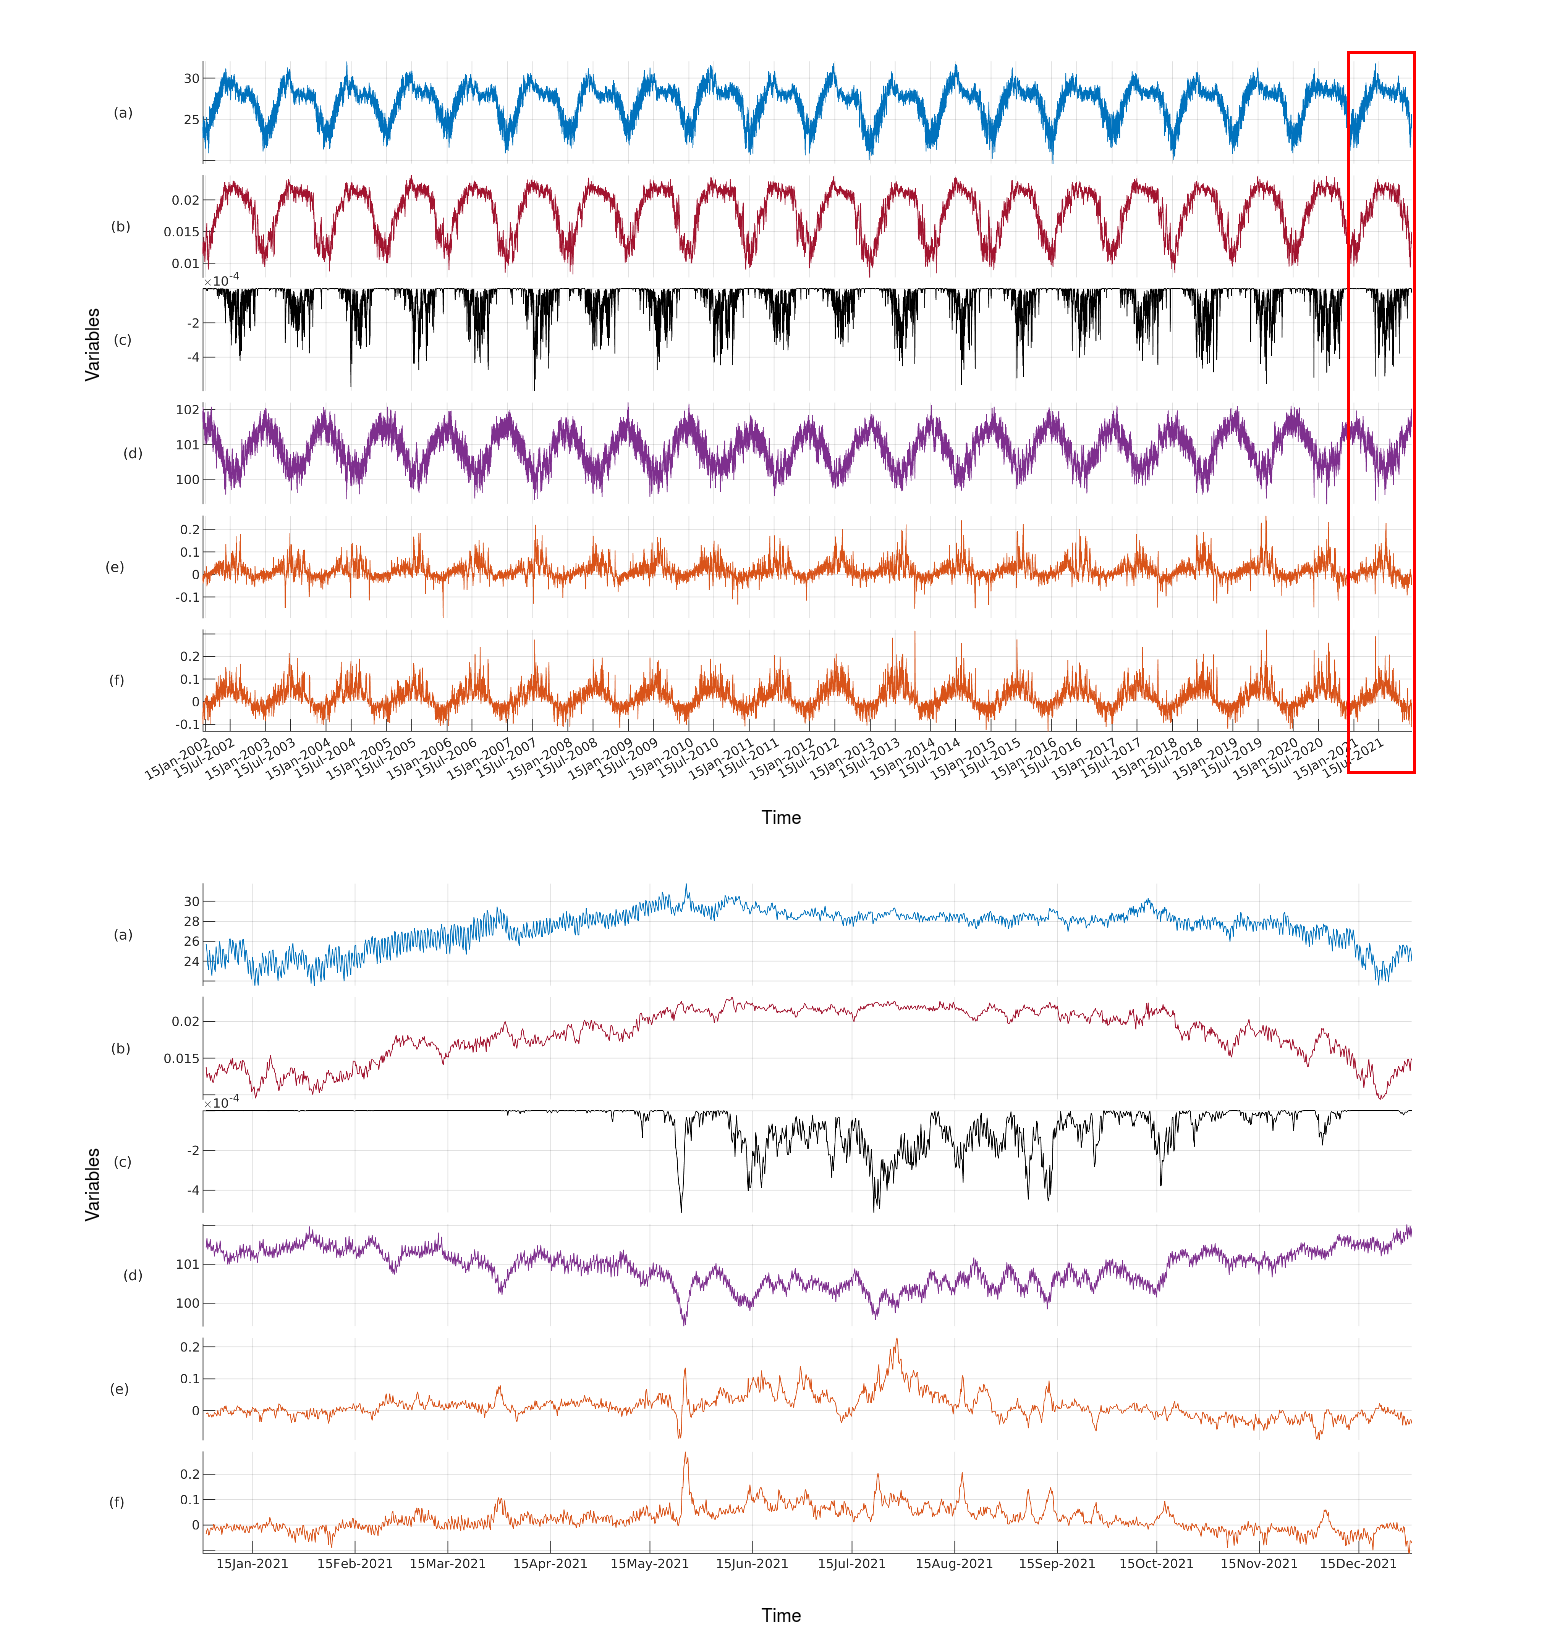
\includegraphics[width=16cm]{contents/final_figure/Figure_5b}
			\caption{Gaya atmosfer pada garis lintang $19^\circ$N dari tahun 2002 hingga 2021, data dari NCEP/NCAR.}
			\label{fig:ncep_2}
		\end{figure}
		
\subsection[Model Iklim]{Model Iklim}
	
		Data selama 20 tahun (2002 - 2021) pada Gambar \ref{fig:ncep_1} dan \ref{fig:ncep_2} diamati untuk menentukan model musiman di kedua domain (lintang $9^\circ$N dan lintang $19^\circ$N) dan bertujuan untuk melihat titik-titik musiman ekstrim setiap tahunnya. Hasil dari model musiman 20 tahun dipotong selama dua tahun terakhir (2020 - 2021) dan disajikan pada Gambar \ref{fig:SM}. Sebagai informasi tambahan, disajikan Tabel \ref{table:extreme} yang merangkum nilai titik ekstrim dari tahun 2002 - 2021 berdasarkan model musiman yang diperoleh.
		
		\begin{table}[H]
			\centering
			\caption{Konstanta dan koefisien prediktor y}
			\label{table:predictor}
			\resizebox{\columnwidth}{!}{%
			\begin{tabular}{|c|ccc|ccc|}
				\hline
				\multirow{2}{*}{Domain} & \multicolumn{3}{c|}{Latitude $9^\circ$N}                                                                               & \multicolumn{3}{c|}{Latitude $19^\circ$N}                                                                              \\ \cline{2-7} 
				& \multicolumn{1}{c|}{$\alpha$} & \multicolumn{1}{c|}{$\beta$} & $\gamma$ & \multicolumn{1}{c|}{$\alpha$} & \multicolumn{1}{c|}{$\beta$} & $\gamma$ \\ \hline
				AirT                    & \multicolumn{1}{c|}{28.125762}             & \multicolumn{1}{c|}{0.219930}             & -0.770494             & \multicolumn{1}{c|}{27.131780}             & \multicolumn{1}{c|}{-0.479135}            & -2.352771             \\ \hline
				SHum                    & \multicolumn{1}{c|}{1.941e-02}             & \multicolumn{1}{c|}{-2.133e-04}           & -8.554e-04            & \multicolumn{1}{c|}{1.811e-02}             & \multicolumn{1}{c|}{-1.194e-03}           & -4.624e-03            \\ \hline
				CPrecR                  & \multicolumn{1}{c|}{-6.752e-05}            & \multicolumn{1}{c|}{2.286e-05}            & 7.285e-06             & \multicolumn{1}{c|}{-5.242e-05}            & \multicolumn{1}{c|}{3.976e-05}            & 6.407e-05             \\ \hline
				SLP                     & \multicolumn{1}{c|}{1.009e+02}             & \multicolumn{1}{c|}{4.803e-02}            & 1.890e-01             & \multicolumn{1}{c|}{1.009e+02}             & \multicolumn{1}{c|}{1.277e-01}            & 6.030e-01             \\ \hline
				TauX                    & \multicolumn{1}{c|}{0.0197177}             & \multicolumn{1}{c|}{-0.0259651}           & -0.0737232            & \multicolumn{1}{c|}{0.0181436}             & \multicolumn{1}{c|}{0.0034581}            & -0.0291363            \\ \hline
				TauY                    & \multicolumn{1}{c|}{0.0189324}             & \multicolumn{1}{c|}{-0.0210637}           & -0.0609275            & \multicolumn{1}{c|}{0.0213336}             & \multicolumn{1}{c|}{0.0037017}            & -0.0511181            \\ \hline
			\end{tabular}%
		}
		\end{table}
		
		Tabel \ref{table:predictor} menunjukkan hasil analisis model musiman dari persamaan (1) untuk gaya atmosfer. Konstanta ($\alpha$) merupakan nilai konstanta yang tidak dipengaruhi oleh musim, sedangkan konstanta ($\beta$) dan ($\gamma$) merupakan variabel yang dipengaruhi oleh musim. Selanjutnya nilai konstanta pada Tabel \ref{table:predictor} dan persamaan (1) menggambarkan model prediksi selama 20 tahun dan hasilnya pada Gambar \ref{fig:SM}.
		
		Nilai rata-rata ($\alpha$) pada Tabel \ref{table:predictor} menunjukkan bahwa nilai AirT lebih besar pada lintang $9^\circ$N dibandingkan pada lintang $19^\circ$N. Hal yang sama terjadi pada variabel SHum dan TauX. Sebaliknya, variabel CPrecR dan TauY lebih besar pada lintang $19^\circ$N daripada lintang $9^\circ$N. Lebih lanjut, untuk variabel SLP nilainya sama di lokasi kedua.
		
		\begin{figure}[H]
			\centering
			\includegraphics[width=15cm]{contents/final_figure/Figure_9}
			\caption{Model musiman untuk pemaksaan atmosfer (a) pada garis lintang $9^\circ$N dan (b) pada garis lintang $19^\circ$N, dari tahun 2020 hingga 2021.}
			\label{fig:SM}
		\end{figure}
	
		Dari Tabel \ref{table:extreme} dan Gambar \ref{fig:SM}, lima gaya yang dikaji - temperature udara 2m (AirT), kelembaban spesifik 2m (SHum), laju presipitasi konvektif (CPrecR), tekanan permukaan laut (SLP), dan tekanan angin U (TauX) dan V ( TauY) - mempengaruhi domain yang diambil sebagai sampel penelitian. Dari kelima variabel tersebut rata-rata nilai ekstrim pada kedua domain terjadi pada bulan Februari dan Agustus setiap tahunnya pada model prediksi yang diperoleh. Tiga parameter AirT, SHum, dan tekanan angin (TauX dan TauY) menunjukkan tren yang sama: minimum di bulan Februari dan maksimum di bulan Agustus. Berbeda dengan tren variabel CPrecR, dan SLP, terlihat bahwa minimum terjadi pada bulan Agustus, dan maksimum terjadi pada bulan Februari. Dari kelima parameter meteorologi yang diperiksa, ekstrim minimum dan maksimum terjadi pada monsun musim dingin dan musim panas.
		
		\begin{table}[H]
			\centering
			\caption{Nilai ekstrim untuk model musiman}
			\label{table:extreme}
			\resizebox{\columnwidth}{!}{%
			\begin{tabular}{|c|c|c|c|c|c|c|l|l|}
				\hline
				Domain                       & Year(s)                       & Extreme & AirT & SHum & CPrecR & SLP & TauX & TauY \\ \hline
				\multirow{4}{*}{2002 - 2021} & \multirow{2}{*}{Latitude $9^\circ$N}  & Min     & Des  & Jan  & Agu    & Jul & Jan  & Jan  \\ \cline{3-9} 
				&                               & Max     & Jun  & Jul  & Feb    & Jan & Jul  & Jul  \\ \cline{2-9} 
				& \multirow{2}{*}{Latitude $19^\circ$N} & Min     & Jan  & Jan  & Jul    & Jul & Jan  & Jan  \\ \cline{3-9} 
				&                               & Max     & Jul  & Jul  & Jan    & Jan & Jul  & Jul  \\ \hline
			\end{tabular}%
		}
		\end{table}
		
\end{spacing}
	
	\vspace{-1pc}
\section[Aplikasi Model]{Aplikasi Model}
\begin{spacing}{1.5}
	\vspace{-1pc}
\subsection[Analisis Chl-a, SST, dan SSS di BoB]{Analisis Chl-a, SST, dan SSS di BoB}
	Gambar \ref{fig:paper1_1}(a) menunjukkan distribusi Chl-a di BoB. Nilai logaritma dari Chl-a dihitung karena nilainya sangat kecil sehingga variasinya menjadi kurang terlihat. Dari hasil logaritma dapat diketahui bahwa nilai Chl-a cukup homogen kecuali pada bagian pantai terutama pada bagian utara BoB. Sebagian besar area permukaan memiliki nilai -1 hingga -2 $mgm^{-3}$. Di sisi lain, di pantai utara BoB, nilai Chl-a bisa mencapai 3 $mgm^{-3}$.
	
	Untuk variabel SST (lihat Gambar \ref{table:paper1_1}(b)), dapat diamati bahwa semakin ke utara menuju pantai, nilai temperature semakin rendah yang ditandai dengan penurunan nilai dari $29^\circ$C menjadi $21^\circ$C. Hal yang sama juga terjadi pada kasus SSS (lihat Gambar \ref{fig:paper1_1}(c)), salinitas di sebagian besar wilayah bernilai 30 Psu, akan tetapi semakin dekat ke pantai utara BoB, nilainya semakin menurun hingga mencapai <20 Psu.
	
	\begin{figure}[H]
		\centering
		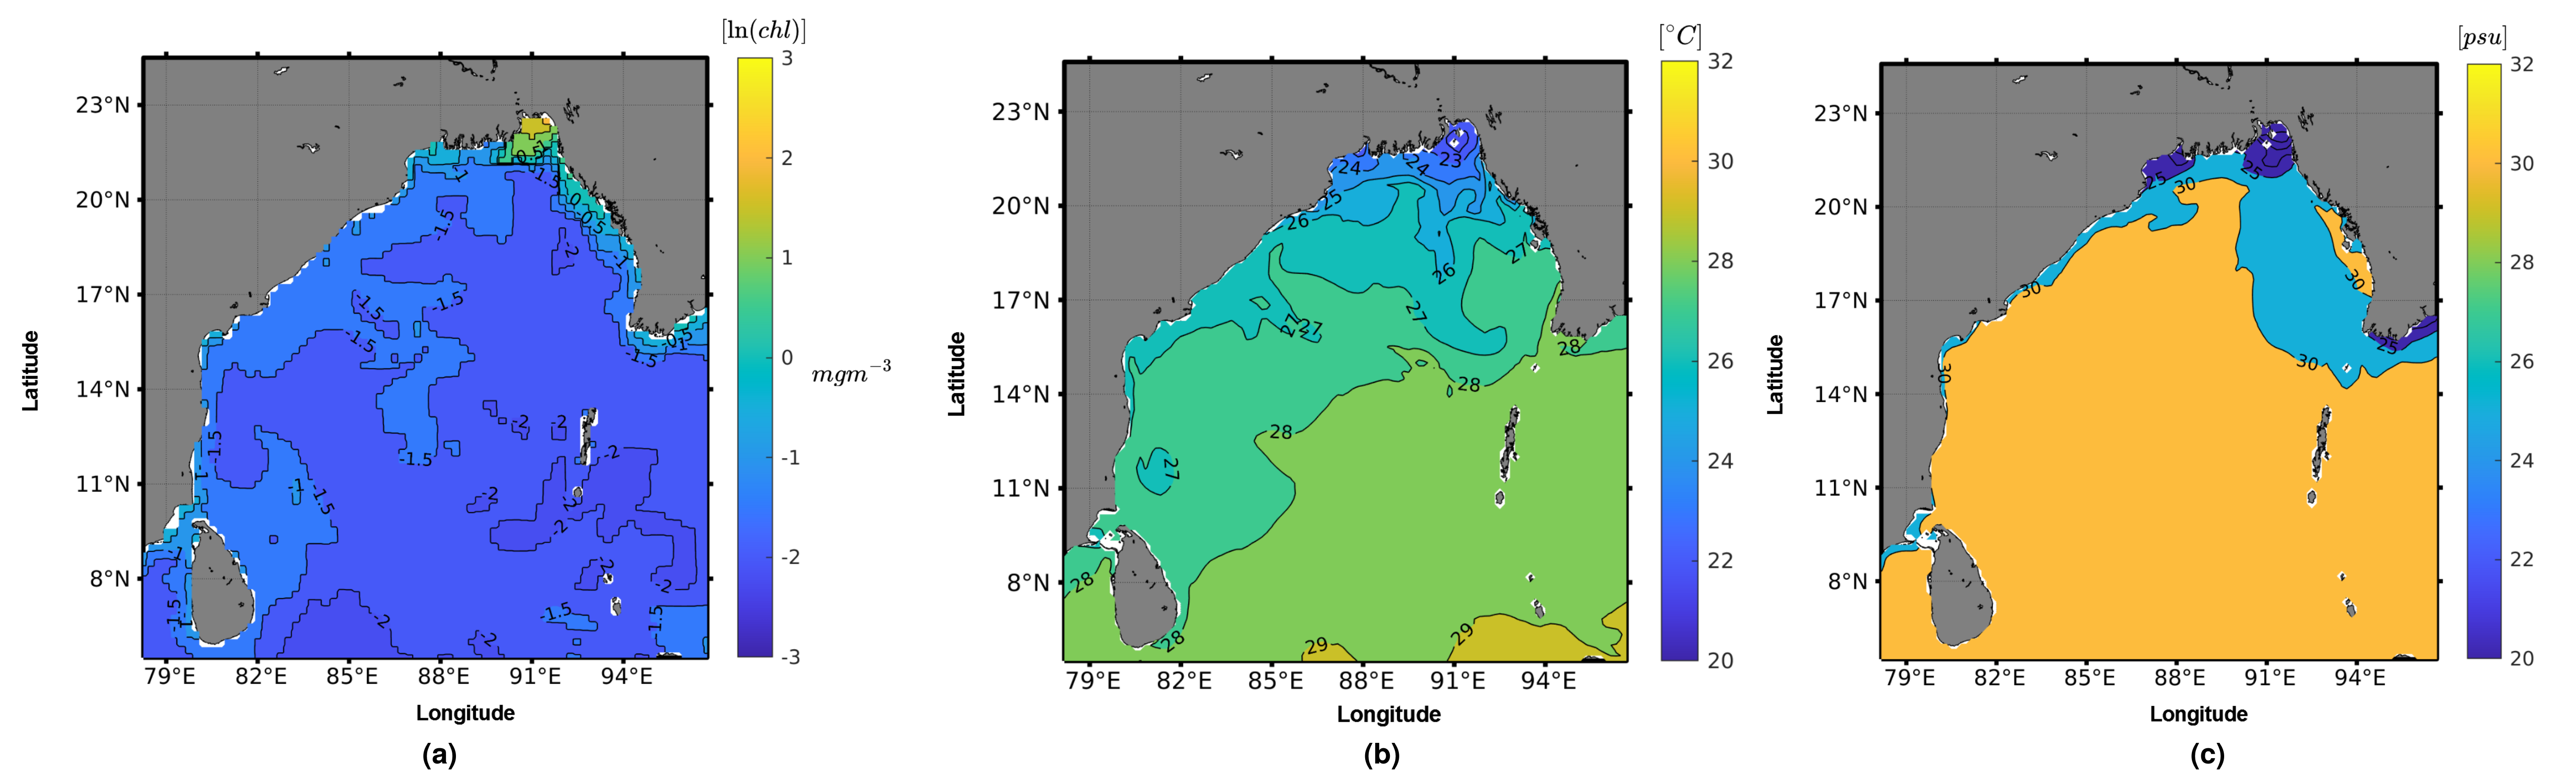
\includegraphics[width=15cm]{contents/final_figure_paper1/gambar_1}
		\caption{(a) Distribusi klorofil-a (Chl-a) (satuan dalam $mgm^{-3}$, nilai logaritmik diambil untuk melihat variasi nilai lebih jelas), (b) Temperature permukaan laut (SST) (satuan dalam $^\circ$C), (c) Salinitas permukaan laut (SSS) (satuan dalam Psu) pada Januari 2021.}
		\label{fig:paper1_1}
	\end{figure}
\subsubsection[Analisis Korelasi]{Analisis Korelasi}
	
	Analisis terhadap 3672 populasi untuk masing-masing variabel (Chl-a, SST, dan SSS) (lihat Tabel \ref{table:paper1_1}) menghasilkan analisis korelasi (lihat Gambar \ref{fig:paper1_2}, tabel uji hipotesis (lihat Tabel \ref{table:paper1_2}), dan tabel analisis varians (lihat Tabel \ref{table:paper1_3}).
	
	Tabel \ref{table:paper1_1} menunjukkan bahwa jumlah terbesar dari 3672 data yang digunakan adalah variabel SSS, diikuti oleh SST dan kemudian Chl-a. Hal yang sama terjadi untuk jumlah rata-rata. Nilai varians terkecil yang ditunjukkan oleh data Chl-a menunjukkan data yang seragam untuk Chl-a. Sedangkan variansi terbesar yang ditunjukkan oleh data SSS menunjukkan data yang cukup bervariasi.
	
	\begin{table}[H]
		\centering
		\caption{Rangkuman data yang digunakan dalam penelitian ini}
		\label{table:paper1_1}
		\begin{tabular}{|c|c|c|c|c|}
			\hline
			Grup  & Banyak & Jumlah   & Rata-rata & Variansi \\ \hline
			Chl-a & 3672   & 893.7106 & 0.243385  & 0.126751 \\ \hline
			SST   & 3672   & 101963.2 & 27.76776  & 1.247772 \\ \hline
			SSS   & 3672   & 117570.7 & 32.01817  & 5.915565 \\ \hline
		\end{tabular}
	\end{table}

	Hasil analisis korelasi pada Gambar \ref{fig:paper1_2}(a-c) menunjukkan bahwa korelasi negatif terjadi pada pasangan Chl-a - SST dan Chl-a - SSS, yang ditunjukkan dengan kemiringan garis regresi negatif (garis biru). Sebaliknya, pasangan SST-SSS menunjukkan korelasi positif yang ditunjukkan dengan kemiringan garis regresi yang positif. Hubungan korelasi negatif menunjukkan bahwa perbandingan nilai antara Chl-a dan SST atau Chl-a dengan SSS berbanding terbalik sehingga jika nilai Chl-a tinggi pada suatu titik koordinat, SST akan memiliki nilai yang rendah pada titik koordinat tersebut. Sebaliknya korelasi positif menunjukkan bahwa perbandingan nilai antara SST dan SSS berbanding lurus sehingga jika nilai SST tinggi pada suatu titik koordinat, maka akan diimbangi dengan nilai SSS yang tinggi pada titik koordinat tersebut.Selanjutnya, evaluasi variasi antara nilai pasangan variabel ditampilkan menggunakan RMSE. Hasilnya adalah pasangan SST - SSS memiliki variasi nilai yang lebih kecil, diikuti oleh Chl-a - SST dan kemudian Chl-a - SSS.
	
	\begin{figure}[H]
		\centering
		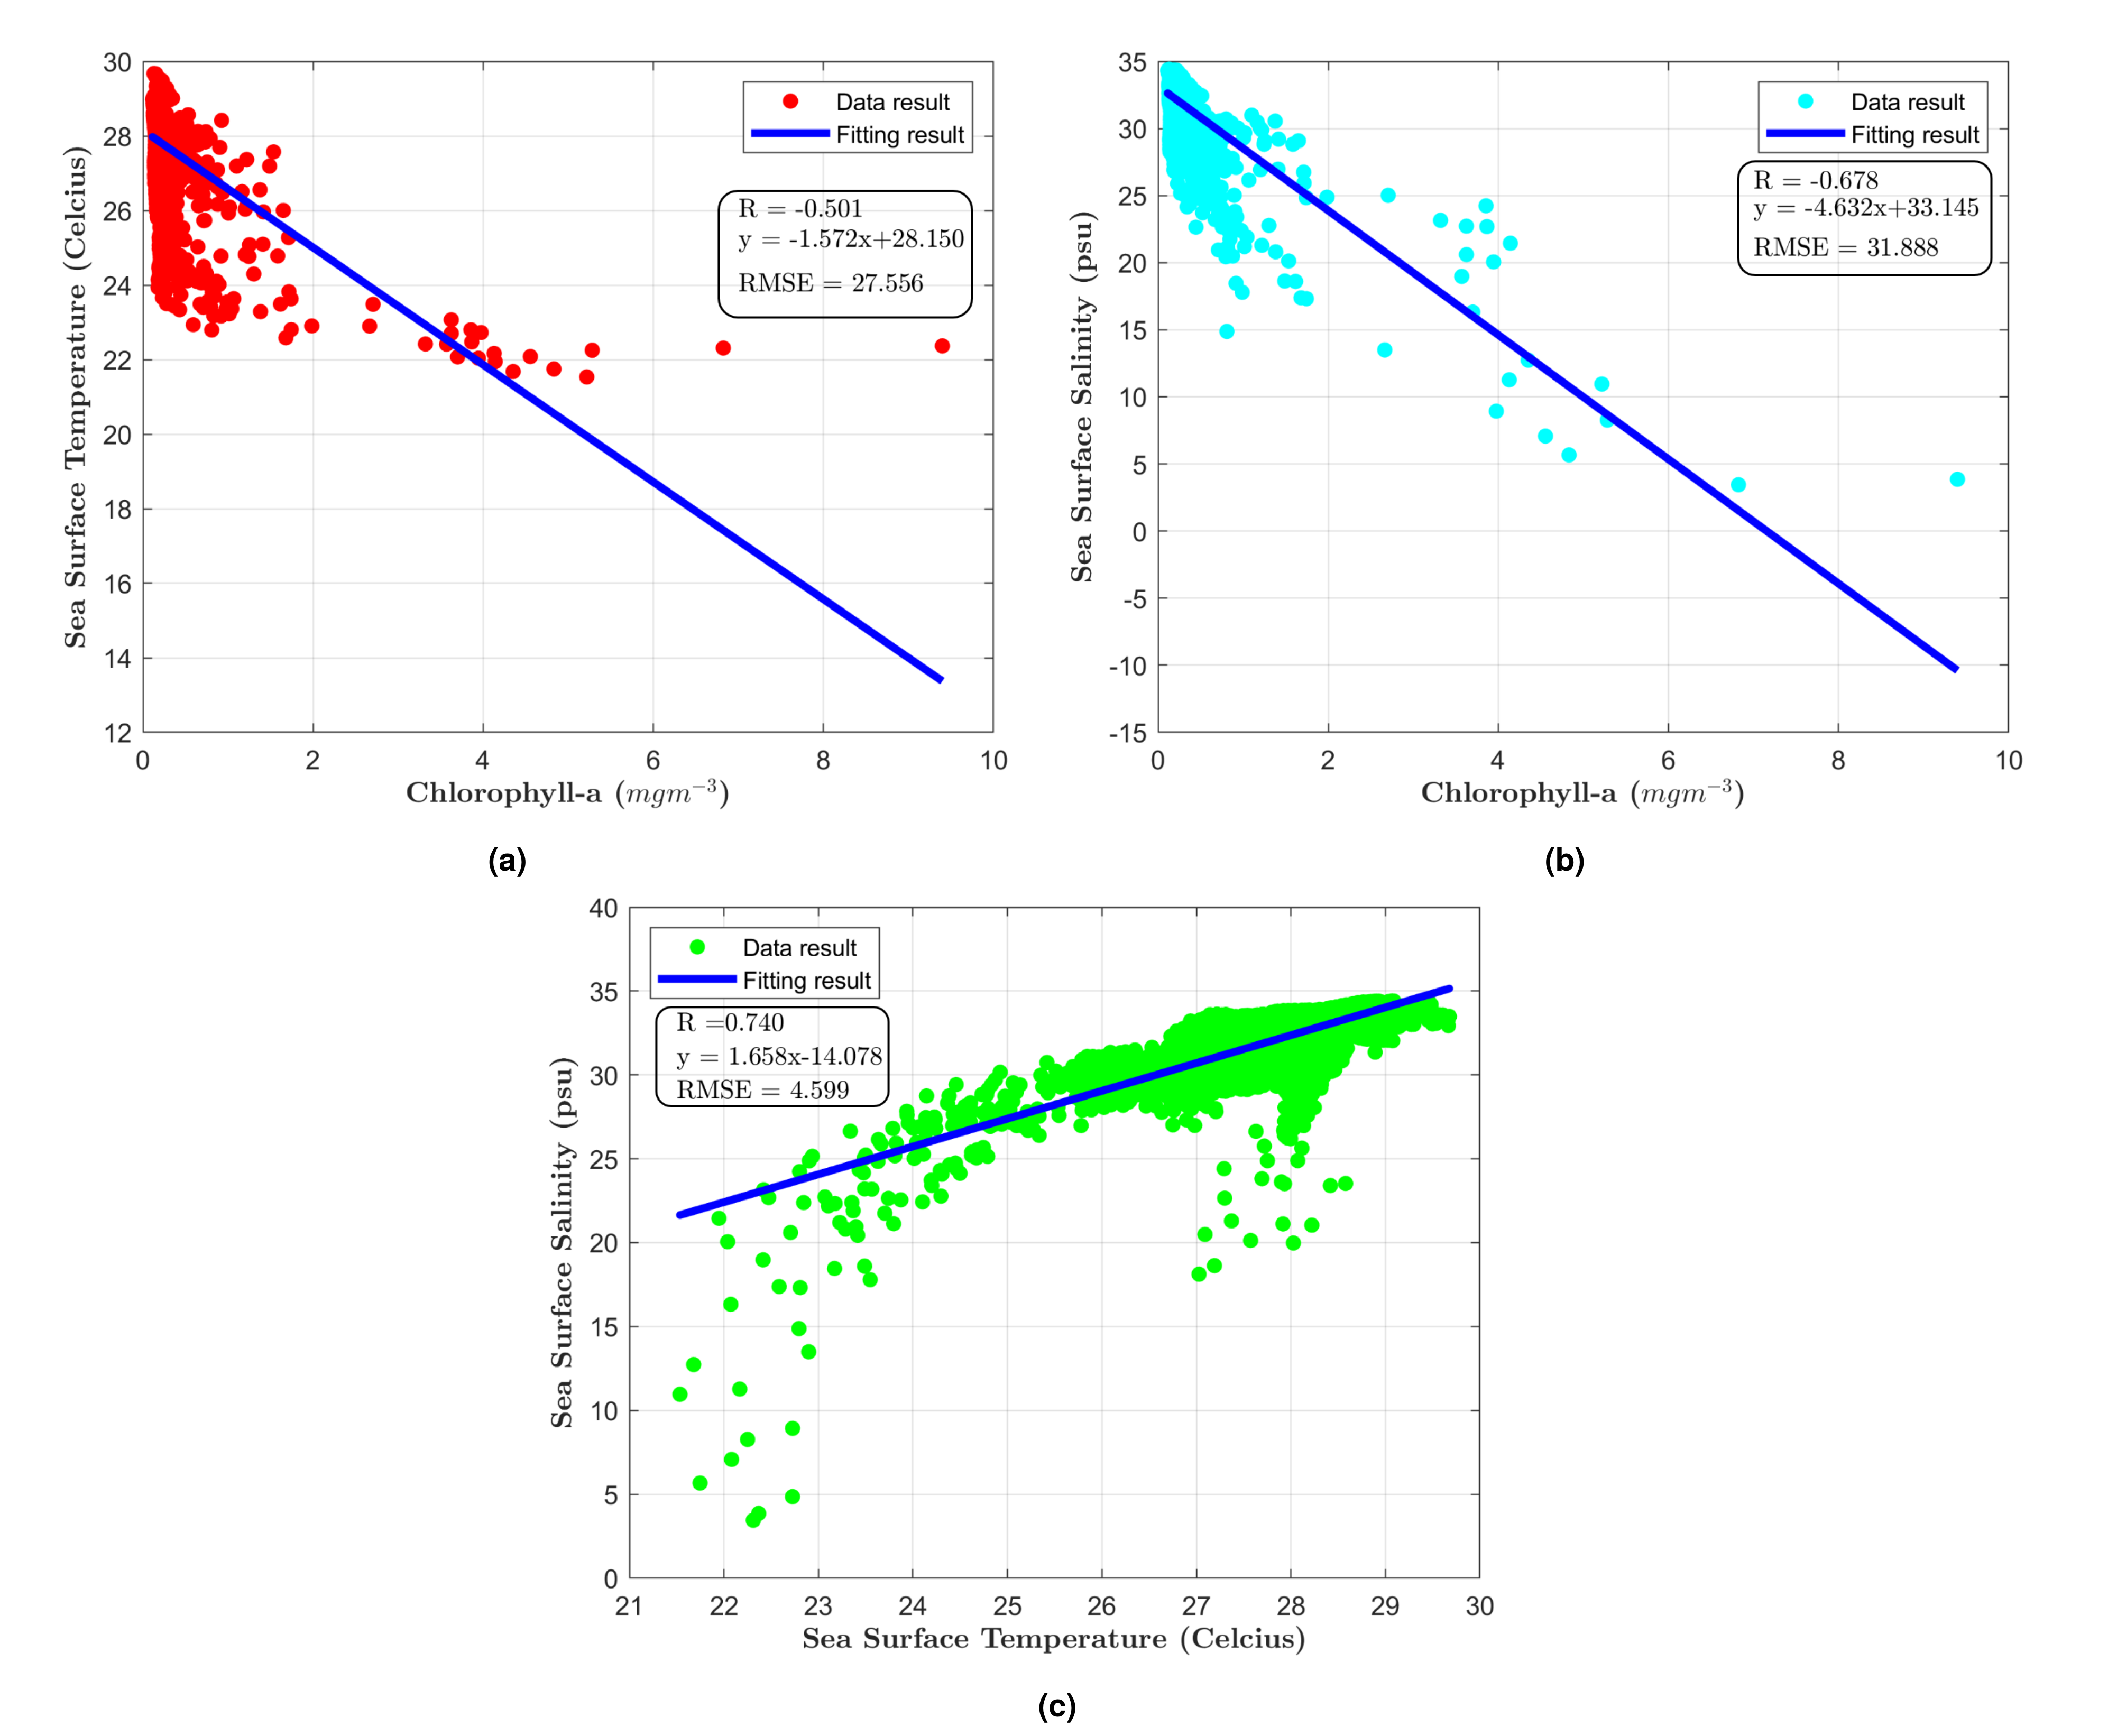
\includegraphics[width=15cm]{contents/final_figure_paper1/gambar_2}
		\caption{Analisis korelasi untuk (a) Klorofil-a - suhu permukaan laut, (b) Klorofil-a - salinitas permukaan laut, dan (c) Suhu permukaan laut - salinitas permukaan laut}
		\label{fig:paper1_2}
	\end{figure}
	
	Gambar \ref{fig:paper1_3} menunjukkan koefisien korelasi dari pasangan variabel yang dibandingkan. Terlihat bahwa pasangan SST - SSS memiliki korelasi paling kuat, diikuti oleh Chl-a - SSS dan kemudian Chl-a - SST. Menurut \shortciteNP{Schober2018}, Chl-a - SST memiliki korelasi sedang dan negatif, Chl-a - SSS memiliki korelasi sedang dan negatif, dan SST - SSS memiliki korelasi yang kuat dan positif. Jika dihitung koefisien determinan, akan diperoleh
	\begin{equation*}
		\begin{aligned}
			r^2_\text{Chl-a - SST}&=0.2511 \;(25.11\%) \\
			r^2_\text{Chl-a - SSS}&=0.4598 \;(45.98\%) \\
			r^2_\text{SST - SSS}&=0.5480 \;(54.8\%) 
		\end{aligned}	
	\end{equation*} 
	Hal ini menunjukkan bahwa kontribusi atau pengaruh Chl-a terhadap SST sebesar 25.11\%, pengaruh Chl-a terhadap SST sebesar 45.98\%, dan pengaruh SST terhadap SSS sebesar 54.8\%. 
	
	\begin{figure}[H]
		\centering
		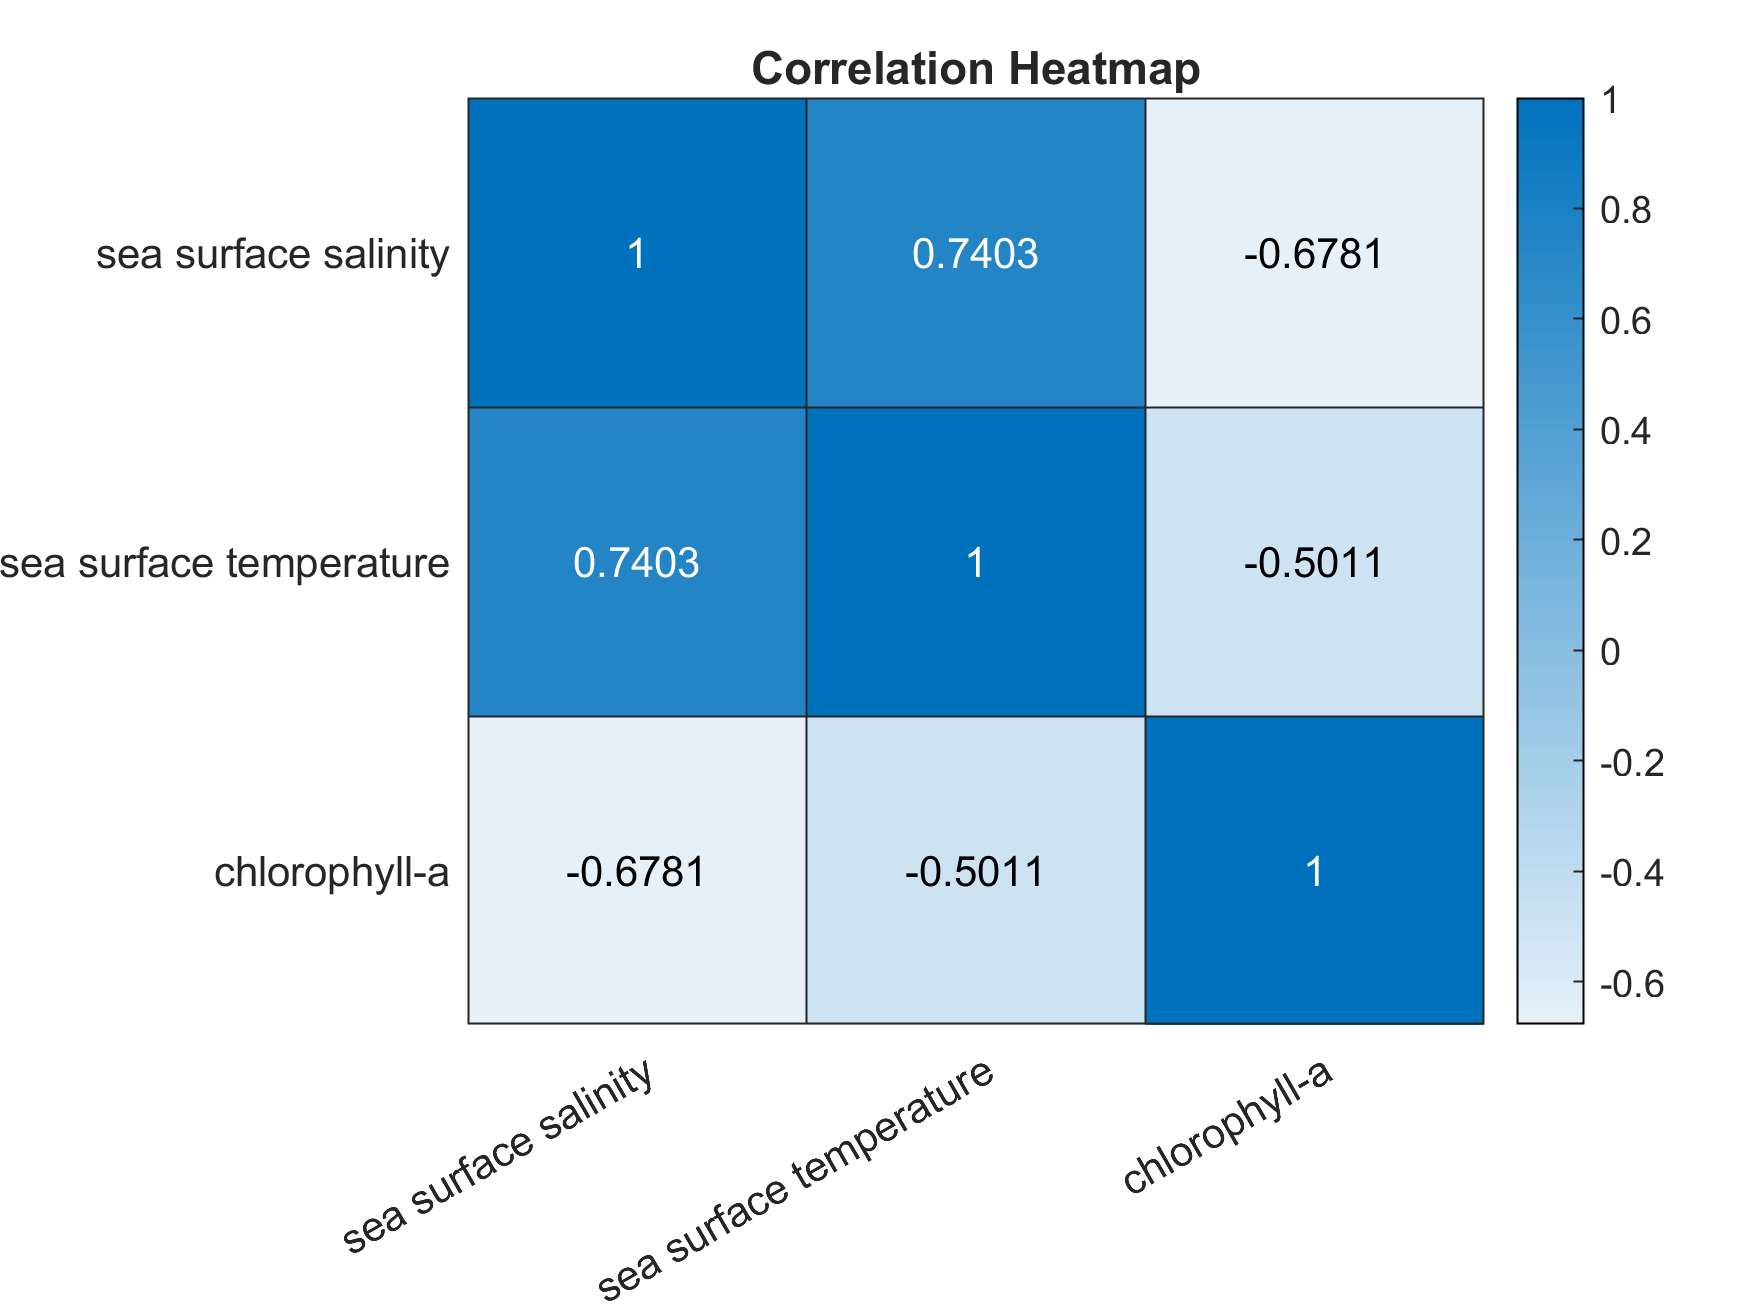
\includegraphics[width=15cm]{contents/final_figure_paper1/gambar_3}
		\caption{Koefisien korelasi (tanpa unit)}
		\label{fig:paper1_3}
	\end{figure}

\subsubsection[Uji Hipotesis dan Analisis Variansi]{Uji Hipotesis dan Analisis Variansi}
	
	Uji hipotesis dilakukan untuk mengetahui apakah koefisien korelasi ($r$) berbeda secara signifikan atau tidak. Berdasarkan hasil pengujian hipotesis pada Tabel \ref{table:paper1_2}, karena 
	\begin{equation*}
		\begin{aligned}
			\{|t_{\text{Chl-a - SST}}|,|t_{\text{Chl-a - SSS}}|,|t_{\text{SST - SSS}}|\}\geq t_{\text{tabel}} \quad \text{dan} \quad \\
			\{|r_{\text{Chl-a - SST}}|,|r_{\text{Chl-a - SSS}}|,|r_{\text{SST - SSS}}|\}\geq r_{\text{tabel}} 	
		\end{aligned}	
	\end{equation*} 
	
	maka hipotesis ($H_o$) bahwa tidak ada hubungan linier antar pasangan variabel, ditolak sehingga terdapat korelasi yang nyata dan negatif untuk pasangan-pasangan Chl-a - SST dan Chl- a - SSS. Di sisi lain, korelasinya nyata dan positif untuk pasangan SST - SSS.
	
	\begin{table}[H]
		\centering
		\caption{Uji hipotesis}
		\label{table:paper1_2}
		\resizebox{\columnwidth}{!}{%
		\begin{tabular}{|c|c|c|c|c|}
			\hline
			Pasangan    & t-nilai & t-tabel ($\alpha=5\%$)                  & r-nilai (koefisien korelasi) & r-tabel ($\alpha=5\%$)               \\ \hline
			Chl-a - SST & -40.535 & \multirow{3}{*}{(0.025; 3670) = 1.9606} & -0.501                       & \multirow{3}{*}{(5\%; 3670) = 0.032} \\ \cline{1-2} \cline{4-4}
			Chl-a - SSS & -76.043  &  & -0.678 &  \\ \cline{1-2} \cline{4-4}
			SST - SSS   & 103.0864 &  & 0.74   &  \\ \hline
		\end{tabular}%
	}
	\end{table}
	Berdasarkan Tabel \ref{table:paper1_3}, karena 
	\begin{equation*}
		\begin{aligned}
			\{|F_{\text{Chl-a - SST}}|,|F_{\text{Chl-a - SSS}}|,|F_{\text{SST - SSS}}|\}\geq F_{\text{tabel}} 	
		\end{aligned}	
	\end{equation*} 
	dan $P-\text{nilai}\leq (\alpha=0.05)$ untuk masing-masing pasangan, dapat disimpulkan bahwa: (1) variabel Chl-a berpengaruh signifikan terhadap variasi nilai variabel SST (2) variabel Chl-a berpengaruh signifikan terhadap variasi nilai variabel SSS, dan (3) variabel SST berpengaruh signifikan terhadap variasi nilai variabel SSS.
	
	\begin{table}[H]
		\centering
		\caption{Analisis variansi (ANOVA)}
		\label{table:paper1_3}
		\resizebox{\columnwidth}{!}{%
		\begin{tabular}{|c|c|c|c|c|c|c|c|}
			\hline
			Pasangan & Sumber Variasi & Jumlah Kuadrat & Derajat Kebebasan & Rata-rata Jumlah Kuadrat & F & P-nilai & F-tabel ($\alpha=5\%$) \\ \hline
			\multirow{3}{*}{Chl-a - SST} & Between Groups & 1390937.466 & 1    & 1390937  & 2023883  & 0 & 3.842726 \\ \cline{2-8} 
			& Within Groups  & 5045.875117 & 7342 & 0.687262 &          &   &          \\ \cline{2-8} 
			& Total          & 1395983.341 & 7343 &          &          &   &          \\ \hline
			\multirow{3}{*}{Chl-a - SSS} & Between Groups & 1853693     & 1    & 1853693  & 613570.5 & 0 & 3.842726 \\ \cline{2-8} 
			& Within Groups  & 22181.34    & 7342 & 3.021158 &          &   &          \\ \cline{2-8} 
			& Total          & 1875875     & 7343 &          &          &   &          \\ \hline
			\multirow{3}{*}{SST - SSS}   & Between Groups & 33169.15    & 1    & 33169.15 & 9260.809 & 0 & 3.842726 \\ \cline{2-8} 
			& Within Groups  & 26296.61    & 7342 & 3.581669 &          &   &          \\ \cline{2-8} 
			& Total          & 59465.76    & 7343 &          &          &   &          \\ \hline
		\end{tabular}%
	}
	\end{table}
	
\subsection[Hubungan antara \textit{Eddies} dan SSH di Samudera Hindia]{Hubungan antara \textit{Eddies} dan SSH di Samudera Hindia}
	
	Angin yang berhembus pada domain penelitian yang ditunjukkan dalam gambar \ref{fig:paper2_1}a tampak tidak begitu teratur dan terlihat bahwa memiliki kondisi yang berbeda di sisi timur laut dan barat daya yang dipisahkan oleh pulau Sumatera. Tampak bahwa di bagian utara domain yang meliputi wilayah bagian laut Cina Selatan, selat Malaka, dan perairan Aceh. Secara umum, di wilayah ini, angin berhembus dari arah timur menuju ke barat. 
	
	Di sisi lain, angin berhembus dari Barat menuju Timur di bagian tengah dan selatan domain yang merupakan wilayah laut lepas samudera Hindia. Dari hasil pengamatan, diketahui bahwa angin paling kencang berada pada bagian laut Cina selatan dan laut lepas samudera hindia dengan nilai kecepatan angin berkisar antara 2 m/s - 6 m/s dan tekanan angin berkisar antara 0.1 Pa - 1.3 Pa. Angin yang tidak begitu kencang mendominasi di wilayah Selat Malaka dan Perairan Barat Aceh dengan kecepatan angin berkisar antara 0.5 m/s - 2.5 m/s dan tekanan angin berkisar antara 0.01 Pa - 0.1 Pa. Penggambaran angin ini sekaligus memvalidasi hasil temuan di Samudera Hindia \shortcite{Schott2001}.
	
	\begin{figure}[H]
		\centering
		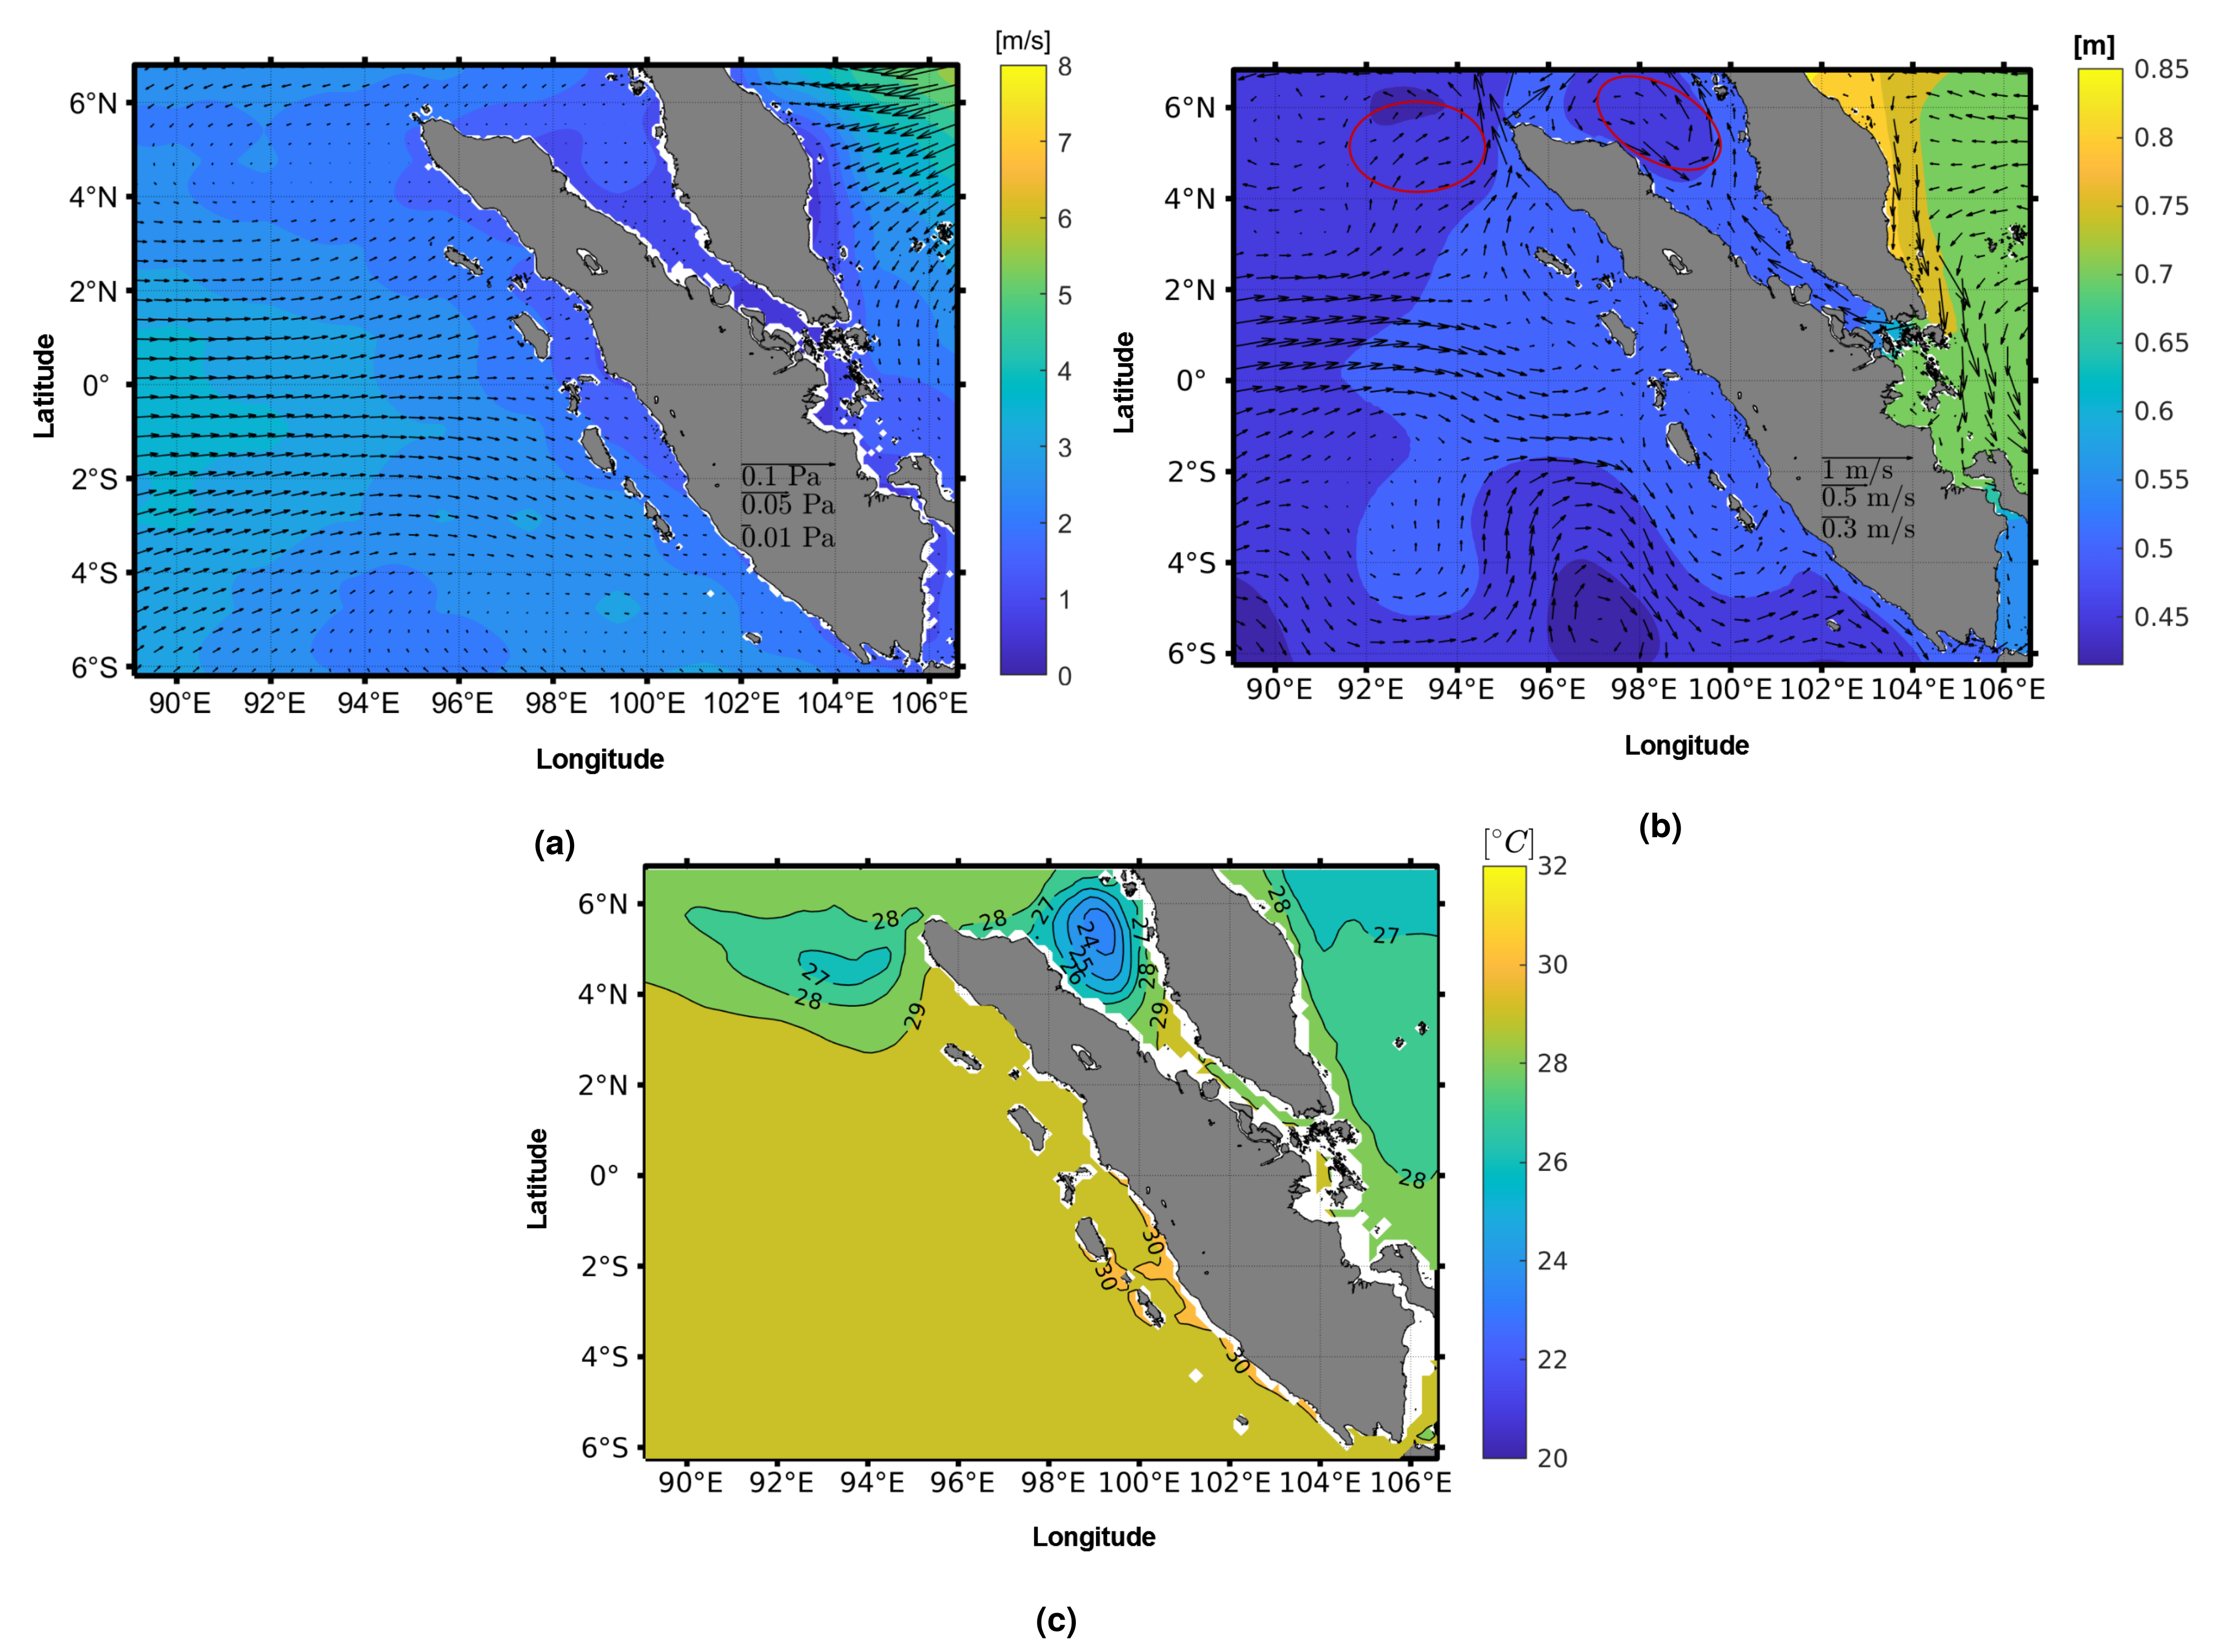
\includegraphics[width=15cm]{contents/final_figure_paper2/gambar_1}
		\caption{(a) Vektor tekanan angin (panah hitam, dalam Pa) dan kecepatan angin (warna, dalam m/s) pada bulan April 2020, (b) Vektor kecepatan arus permukaan laut (UV) (panah hitam, dalam m/s) dan Ketinggian permukaan laut di atas geoid (SSH) (warna, dalam m/s) pada bulan April 2020. Lingkaran merah menunjukkan lokasi pusaran yang terjadi dan (c) Temperature potensial air laut permukaan (SST) (warna, dalam $^\circ$C) pada bulan April 2020.}
		\label{fig:paper2_1}
	\end{figure}
	
	Dalam Gambar \ref{fig:paper2_1}b, tampak bahwa perbedaan nilai SSH sangat kontras terjadi. Nilai SSH lebih tinggi di bagian laut Cina Selatan dibandingkan wilayah domain yang lain. Dari hasil SSH yang digambarkan tampak bahwa, SSH yang rendah muncul disekitar lokasi pusaran. Pusaran (\textit{Eddies}) terjadi dibeberapa titik lokasi dalam penelitian khususnya yang bersesuaian dengan bagian belahan bumi Utara (\textit{Northern Hemisphere}), yaitu Selat Malaka pada koordinat ($98^\circ$E, $6^\circ$N), dan Perairan Aceh pada koordinat ($93^\circ$E, $5^\circ$N). Kedua titik lokasi pusaran yang terjadi memiliki arah arus yang berlawanan arah jarum jam. Sirkulasi laut yang dipengaruhi oleh angin mengakibatkan terjadinya pusaran yang berlawanan arah jarum jam. Aliran pada lapisan permukaan Ekman di kedua titik lokasi pusaran berasosiasi dengan perilaku angin dan memiliki karakteristik divergent yang mendorong gerakan vertikal dari bawah ke atas (peristiwa \textit{upwelling}) \shortcite{10.2307/24805614}. Fenomena ini membawa air dengan konsentrasi tinggi nutrisi seperti nitrat dan fosfat ke permukaan laut. Perairan yang kaya nutrisi ini menjadi pendorong bagi pertumbuhan plankton dan ganggang mikroskopis di perairan tersebut. Karena air dari kedalaman yang dibawa ke permukaan seringkali mengandung kandungan nutrisi yang tinggi, upwelling dapat membantu pertumbuhan rumput laut dan plankton. Selanjutnya, rumput laut dan plankton menjadi penyedia sumber makanan bagi ikan-ikan, mamalia laut, dan burung-burung di daerah tersebut.
	
	Kedua pusaran pada wilayah Selat Malaka dan Perairan Aceh yang diidentifikasi oleh SSH memiliki kesesuaian dengan fenomena SST yang rendah pada lokasi terjadinya pusaran. Hal ini ditunjukkan pada Gambar \ref{fig:paper2_1}c, dimana pada wilayah selat Malaka nilai SST berkisar antara $24^\circ$C - $28^\circ$C dan bernilai semakin rendah seiring menuju ke pusat pusaran. Untuk wilayah perairan Aceh, nilai SST berkisar antara $27^\circ$C - $28^\circ$C dan nilai terendah berada di pusat pusaran.
\end{spacing}